\documentclass[tikz, varwidth=true]{standalone}
\begin{document}
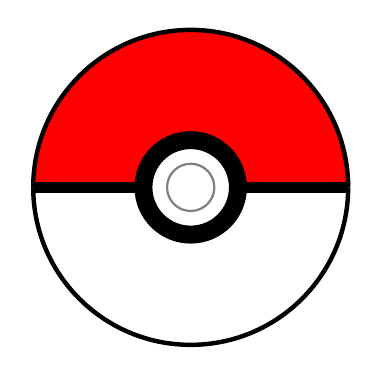
\begin{tikzpicture}[font=\small\sffamily, >=latex, thick]

	%% draw help lines
	% \draw[step=0.5, help lines] (-2.4,-2.4) grid (2.4,2.4);

	\filldraw [ultra thick, fill = red] (2.0,0) arc [start angle = 0, end angle = 180, radius = 2.0] ;
	\filldraw [ultra thick, fill = white] (-2.0,0) arc [start angle = 180, end angle = 360, radius = 2.0] ;

	\draw[line width=4.0] (-2.0,0) -- (2.0,0);

	\filldraw[fill=black] (0,0) circle [radius = 0.7];
	\filldraw[fill=white] (0,0) circle [radius = 0.5];
	\draw[gray] (0,0) circle [radius = 0.3];

\end{tikzpicture}
\end{document}
